\documentclass{patmorin}
\usepackage{pat}
\usepackage{amsopn}

\DeclareMathOperator{\obs}{obs}
\newcommand{\x}{\mathsf{x}}
\newcommand{\y}{\mathsf{y}}

\title{On Obstacle Numbers}
\author{Bellairs Geometry and Graphs 2013}

\begin{document}
\maketitle

\begin{abstract}
The obstacle number of a graph is a new graph parameter
introduced by Alpert, Koch, and Laison (2010).  Pach \etal\ (2012)
show that there exist graphs with $n$ vertices having obstacle
number in $\Omega(n/\log n)$. In this paper we up this lower bound to
$\Omega(n/(\log\log n)^2)$
\end{abstract}

\newpage

\section{Introduction}

The obstacle number of a graph is a new graph parameter introduced by
Alpert, Koch, and Laison \cite{alpert.koch.ea:obstacle}.  Let $G=(V,E)$ be
a graph, let $\varphi:V\to \R^2$ be a one-to-one mapping of the vertices
of $G$ onto $\R^2$, and let $S$ be a set of connected subsets of $\R^2$.
The pair $(\varphi,S)$ is an \emph{obstacle representation} of $G$ if and
only if, for every pair of vertices $u,w\in V$, the edge $uw\in E$ if and
only if the open line segment with endpoints $\varphi(u)$ and $\varphi(w)$
does not intersect any \emph{obstacle} in $S$.  When $uw\not\in E$
we call $uw$ a \emph{non-edge} of $G$. The \emph{obstacle number} of a
graph $G$, denoted by $\obs(G)$, is the minimum number of obstacles in
any obstacle representation of $G$.

An $h$-obstacle representation of $G$ is an obstacle representation with
at most $h$ obstacles.  The (point set which is the) image of $\varphi$
in an obstacle representation is said to \emph{support} the obstacle
representation.  \figref{fivebyfive} shows a surprising example of a
1-obstacle representation of the $5\times 5$ grid graph.  Since at least
one obstacle is necessary to represent any graph other than a complete
graph, this proves that the $5\times 5$ grid graph has obstacle number 1.

\begin{figure}
  \begin{center}
    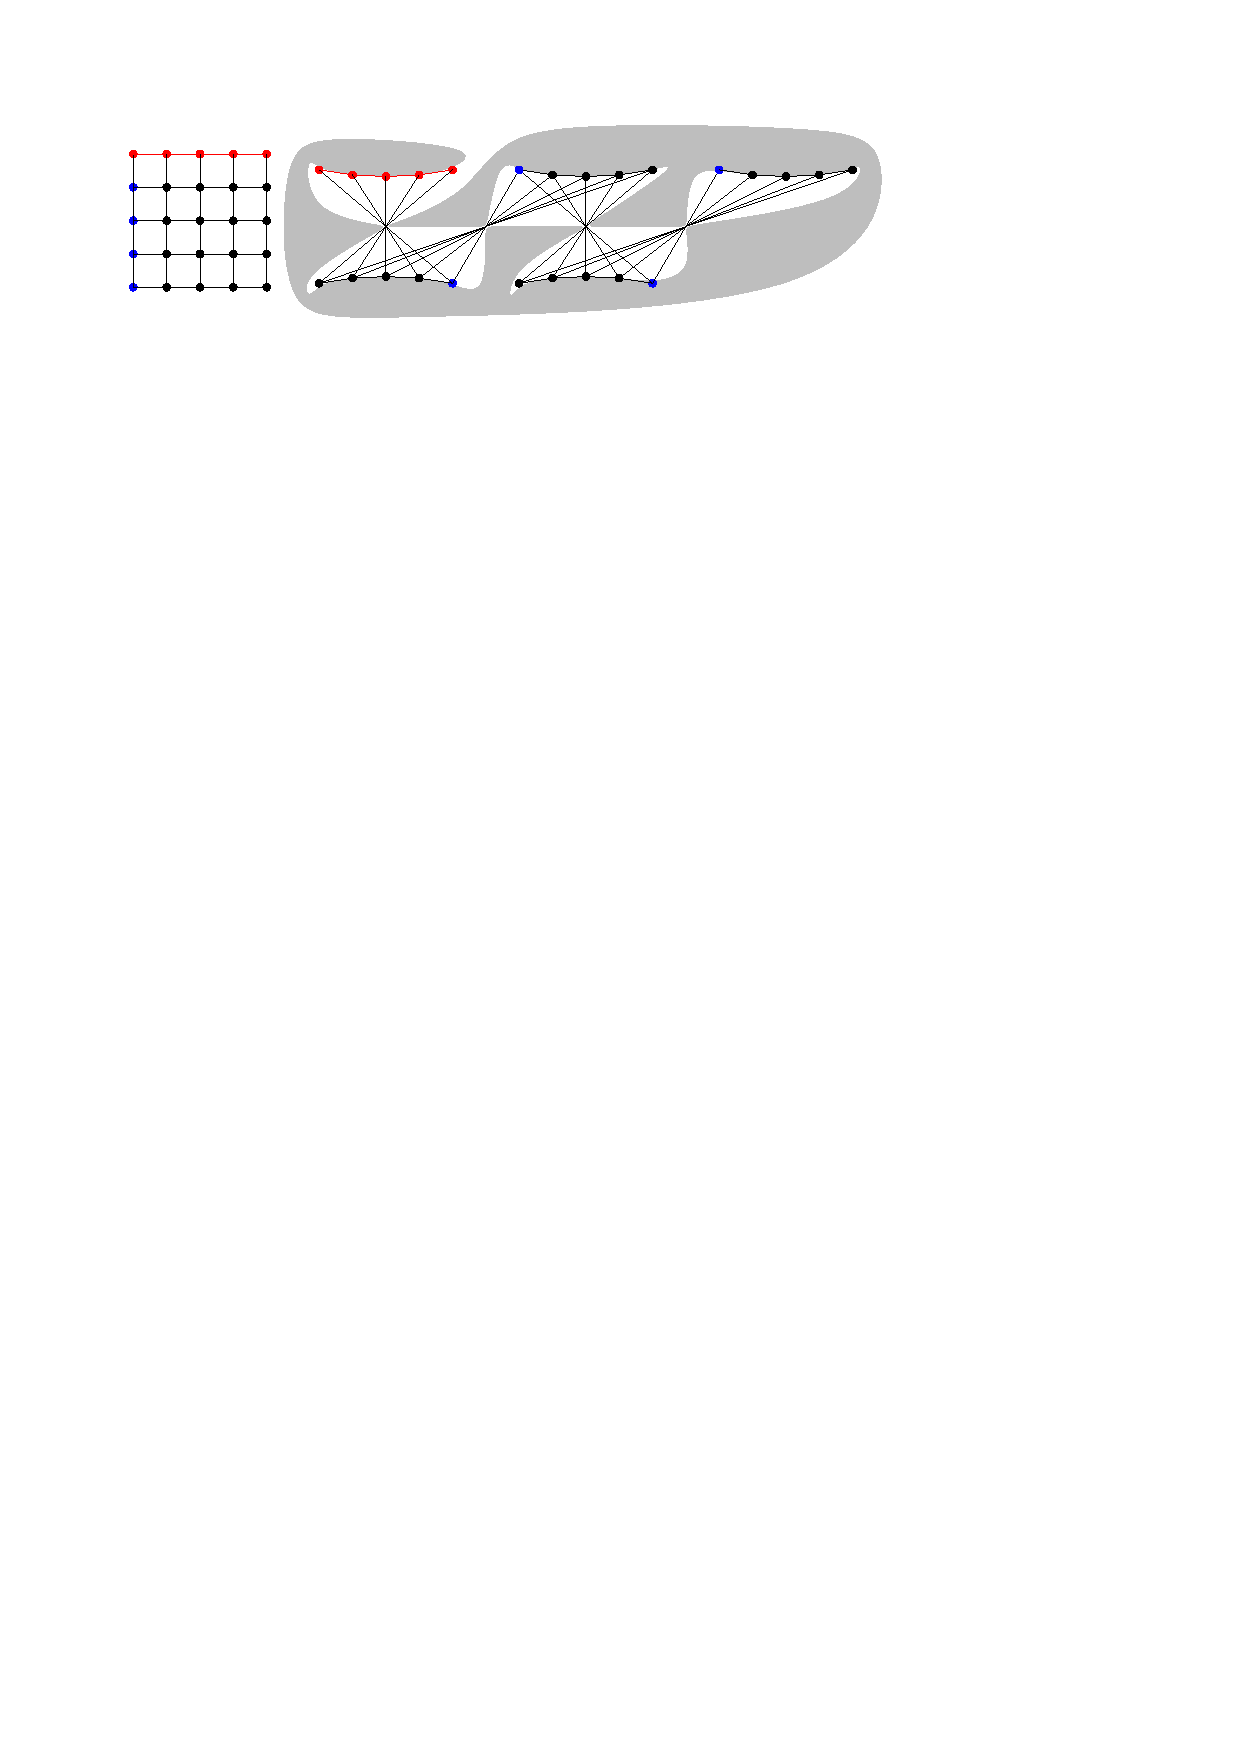
\includegraphics{fivebyfive}
  \end{center}  
  \caption{The $5\times 5$ grid graph has obstacle number 1.}
  \figlabel{fivebyfive}
\end{figure}

Since their introduction, obstacle numbers have generated a significant
amount of research interest 
\cite{%
   fulek.saeedi:convex,%
   johnson.sarioz:computing,%
   mukkamala.pach.ea:lower,%
   mukkamala.pach.ea:graphs,%
   pach.sarioz:small,%
   pach.sarioz:on,%
   sarioz:approximating%
}.
A fundamental---and far from answered---question about obstacle numbers
is that of determining the \emph{worst-case obstacle number},
\[
    w(n) = \max \{\obs(G) :\mbox{$G$ is a graph with $n$ vertices}\}
    \enspace ,
\] 
of a graph with $n$ vertices.

The worst-case obstacle number is obviously upper-bounded by
$\binom{n}{2}\in O(n^2)$ since, by mapping the vertices of $G$
 onto a point set in sufficiently general position, one can place
a small obstacle---even a single point---on the mid-point of each non-edge
of $G$.  No upper-bound on $w(n)$ that is asymptotically better than
$O(n^2)$ is known.

More is known about lower-bounds on $w(n)$.  Alpert \etal\
initially show that the worst-case obstacle number is
$\Omega(\sqrt{\log n})$.\note{Double-check this. I took it
from \cite{mukkamala.pach.ea:graphs}, but I think it should be
$\Omega(\sqrt{\log n/\log\log n}$.}
%\footnote{Alpert \etal's lower-bound uses the Erd\"os-Szekeres convex
%$n$-gon theorem and shows the existence of an $n$-vertex graph $G$
%with $\obs(G)\ge \sqrt{\log n/\log\log n}$.}
Pach \etal\ \cite{mukkamala.pach.ea:graphs} showed that
$w(n)\in \Omega(n/\log^2 n)$.
Mukkamala \etal\ \cite{mukkamala.pach.ea:lower} later increased this
to $w(n)\in\Omega(n/\log n)$.  In the current paper, we up the lower-bound
again by proving the following theorem:
\begin{thm}\thmlabel{main}
  For every integer $n>0$, $w(n)\in\Omega(n/(\log\log n)^2)$, i.e., there
  exists a graph $G$ with $n$ vertices and $\obs(G)\in\Omega(n/(\log\log
  n)^2)$.
\end{thm}

\section{The Proof}

Our proof strategy is an application of the probabilistic method
\cite{alon.spencer:probabilistic}.  We will show that, for a random graph,
$G$, with a fixed embedding, the probability, $p$, that this embedding
allows for an obstacle representation with few obstacles is extremely
small.  We will then show that the number, $N$, of combinatorially
distinct embeddings is not too big.  Small and big in this case are
defined so that $pN < 1$.  Therefore, by the union bound, there exists at
least one graph, $G'$, that has no embedding that allows for an obstacle
representation with few obstacles.  In other words, $\obs(G')$ is large.

\subsection{A Random Graph with a Fixed Embedding}

We make use of the following theorem, due to Mukkamala, Pach, and
P\'alv\"olgyi \cite{mukkamala.pach.ea:lower} about the number of $n$
vertex graphs with obstacle number at most $h$:
\begin{thm}[Mukkamala, Pach, and P\'alv\"olgyi 2012]\thmlabel{pach-gang}
  For any $h\ge 1$, the number of graphs having $m$ vertices and
  obstacle number at most $h$ is at most $2^{O(hn\log^2 n)}$.
\end{thm}

The following lemma shows that, for random graphs, a fixed point
set and fixed embedding is \emph{very} unlikely to yield an obstacle
representation with few obstacles.

\begin{lem}\lemlabel{fixed}
  Let $G=(V,E)$ be an Erd\"os-R\'enyi random graph $G_{n,\frac{1}{2}}$,
  let $P\subset\R^2$ be a set of $n$ points, let
  $\varphi:V\rightarrow P$ be a bijection between $V$ and $P$ that is
  independent of the choices of edges in $G$, and let $(\varphi, S)$ be
  an obstacle representation of $G$ using the minimum number of obstacles
  (subject to $G$ and $\varphi$).  Then, for any constant $c>0$,
  \[
     \Pr\{|S| \in \Omega(n/(\log\log n)^2) \ge 1-e^{-\Omega(cn\log n)}  \enspace .
  \] 
\end{lem}

\begin{proof}
Fix some integer $k$ to be specified later and first consider some
arbitrary subset $P'\subset P$ of $k$ points and let $G'=(V',E')$
be the subgraph of $G$ induced by the set $V'=\{\varphi^{-1}(x):x\in
P'\}$ of vertices that are mapped by $\varphi$ to $P'$.  Applying
\thmref{pach-gang} with $n=k$ and $h=\alpha k/\log^2 k$, we obtain
\begin{equation}
     \Pr\{\obs(G') \le \alpha k/\log^2 k\} 
       \le \frac{2^{O(\alpha n^2)}}{2^{\binom{k}{2}}}
       = e^{-\Omega(k^2)} \enspace , \eqlabel{g1}
\end{equation}
for a sufficiently small constant $\alpha > 0$.  Note that, if
$\obs(G')\ge h$, then, in the obstacle representation $(\varphi,S)$,
there must be at least $h-1$ obstacles of $S$ that are contained in the
convex hull of $P'$.

Without loss of generality assume that no two points in $P$ have the
same x-coordinate and denote the points in $P$ by $x_0,\ldots,x_{n-1}$
by increasing order of x-coordinate.  Let $m=\lfloor n/k\rfloor$ and
consider the point sets $P'_0,\ldots,P'_{m-1}$, where
\[ 
  P_i'=\{x_{ik},x_{ik+1},\ldots,x_{ik+k-1}\} \enspace .
\]  
That is, $P_0',\ldots,P_{m-1}'$ are determined by vertical slabs,
$s_0,\ldots,s_{m-1}$ that each contain $k$ points.  \Eqref{g1} shows
that, with probability at least $1-2^{-\Omega(k^2)}$, the obstacle number
of the subgraph that maps to $P'_i$ is $\Omega(k/\log^2 k)$.  If this
occurs, then $S$ has $\Omega(k/\log^2 k)$ obstacles that are completely
contained in the slab $s_i$.  These obstacles are therefore disjoint
from any other obstacles contained in any other slab $s_j$, $j\neq i$.

We are proving a lower bound on the number of obstacles, so we are
worried about the case where the number of slabs that do \emph{not}
completely contain at least $\alpha k/\log^2 k$ obstacles exceeds $m/2$.
The number of slabs, $M$, not containing at least $\alpha k/\log^2 k$
obstacles is dominated by a binomial$(m,2^{-\Omega(k^2)})$ random
variable.  Using Chernoff's bound on the tail of a binomial random
variable,\footnote{%
  Chernoff's Bound: For any binomial$(m,p)$ random variable, $B$,
  any $\delta>0$ and $\mu=mp$, 
  \[ \Pr\{B\ge (1+\delta)\mu\}
     \le \left(\frac{e^{\delta}}{(1+\delta)^{1+\delta}}\right)^{\mu} 
       \enspace . 
  \]}
we have that
\begin{align*}
  \Pr\{M \ge m/2\} & = \Pr\{M\ge (1+\delta)\mu\}
    & \text{(where $\mu=me^{-ck^2}$ and $\delta=e^{ck^2-1}-1$)} \\
    & \le \left(\frac{e^{\delta}}{(1+\delta)^{1+\delta}}\right)^{\mu} \\
    & = \left(\frac{e^{e^{ck^2}}}{(e^{ck^2-1})^{e^{ck^2-1}}}\right)^{me^{-ck^2}}\\
    & = \left(\frac{e^{e^{ck^2}}}{e^{(ck^2-1)e^{ck^2-1}}}\right)^{me^{-ck^2}}\\
    & = \frac{e^{m}}{e^{m(ck^2-1)e^{ck^2-1}e^{-ck^2}}} \\
    & = \frac{e^{m}}{e^{m(ck^2-1)/e}} \\
    & = e^{-\Omega(mk^2)} \enspace .
\end{align*}
Taking $k=\sqrt{c}\log n$ and recalling that $m=\lfloor n/k\rfloor$, we obtain
the desired result.  In particular,
\[
    |S| \ge \Omega\left(\left(k/\log^2 k\right)\times m \right)
      = \Omega\left(n/(\log\log n)^2\right)
\]
with probability at least
\[
    1-e^{-\Omega(mk^2)} = 1-e^{-\Omega(cn\log n)} \enspace . \qedhere
\]
\end{proof}

We have completed the first step in our application of the probabilistic
method.  \lemref{fixed} shows that the probability, $p$, that a
particular embedding of the random graph $G$ is able to yield an obstacle
representation with $o(n/(\log\log n)^2)$ obstacles is extremely small.
The remaining difficulty is establishing a sufficiently strong upper-bound
on $N$, the number of embeddings of $G$. In actuality, the number of
embeddings is uncountable.  However, we are interested in the number of
``combinatorially distinct'' embeddings.  In particular, we would like
to partition the set of embeddings into equivalence classes such that,
within each equivalence class, the minimum number of obstacles in an
obstacle representation remains the same.

Classifying embeddings (labelled sets of $n$ points) into combinatorially
distinct equivalence classes has been considered previously. Several
definitions of equivalence exist, including oriented matroid (a.k.a.,
chirotope) equivalence
\cite{bland.vergnas:orientability,folkman.lawrence:oriented},
semispace equivalence \cite{goodman.pollack:semispaces}, order equivalence
\cite{goodman.pollack:multidimensional}, and combinatorial equivalence
\cite{goodman:on,goodman.pollack:semispaces}.  For the latter two
definitions of equivalence, the number of distinct (equivalence classes
of) point sets is $e^{O(n\log n)}$ \cite{goodman.pollack:upper}.

%Definitions include equivalence classes of point
%sets with the same \emph{order type} \cite{goodman.pollack:upper}, in which the orientation
%of every triple of points is preserved and equivalence classes of point
%sets with the same \emph{combinatorial-type}, in which a labelled point
%set is identified with the periodic sequence of permutations obtained
%by orthogonally projecting the points onto a line that rotates around
%a fixed point \cite{goodman.pollack:}.  Under both definitions, the number of distinct
%(equivalence classes of) point sets is $e^{O(n\log n)}$

Unfortunately, neither order types nor combinatorial-types are
sufficient for answering questions about obstacle representations.
To see this, consider the two embeddings of the same graph shown in
\figref{order-type-problem}.  These two embeddings have the same order
type and the same combinatorial type. However, the embedding on the right
admits an obstacle representation with one obstacle, while the one on
the left requires two obstacles. To see why this is so, observe that
each embedding needs an obstacle on the outer face (shown) while the one
on the left needs an additional obstacle inside one of the inner faces.

\begin{figure}
  \begin{center}
    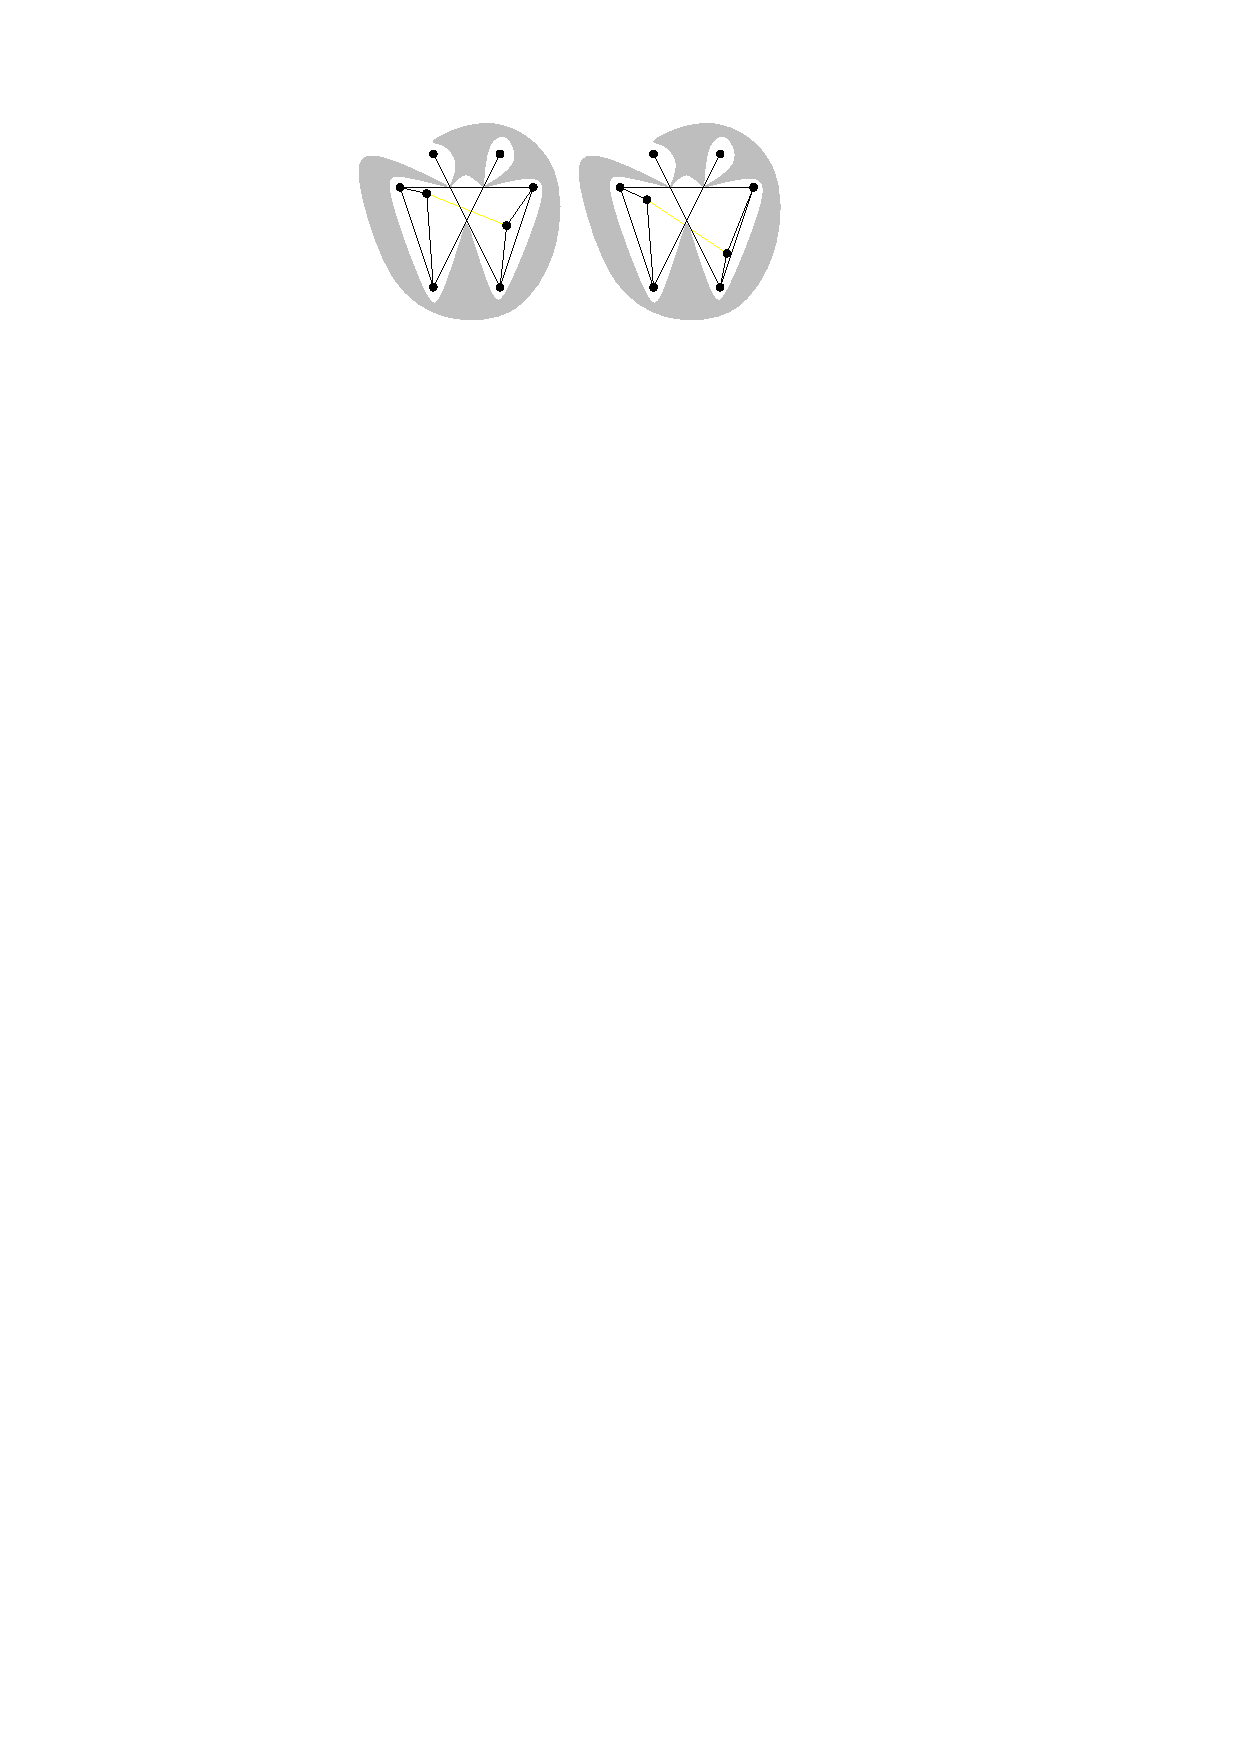
\includegraphics{order-type}
  \end{center}
  \caption{Order type and combinatorial type are insufficient to determine 
      the number of obstacles needed in an obstacle representation.}
  \figlabel{order-type-problem}
\end{figure}

\subsection{Super-Order Types}

We now define an equivalence relation on point sets that works for our
purposes.  Consider a sextuple $S=\langle a_1,a_2,b_1,b_2,c_1,c_2\rangle$
of points with $a_1\neq a_2$, $b_1\neq b_2$, $c_1\neq c_2$, and 
$\{a_1,a_2\}\cap\{b_1,b_2\}\cap\{c_1,c_2\}=\emptyset$.  Let $A$
denote the directed line through $a_1$ and $a_2$ that is directed from
$a_1$ towards $a_2$. Define $B$ and $C$ similarly, but with respect to
$b_1,b_2$ and $c_1,c_2$, respectively.  We say that the sextuple, $S$,
is \emph{degenerate} if
\begin{enumerate}
  \item any of $A$, $B$, or $C$ is vertical;
  \item $A$ is parallel to $B$ or to $C$; or
  \item $A$, $B$, and $C$ contain a common point.
\end{enumerate}
We define the \emph{type}, $\sigma(S)$, of $S$ as
\[
    \sigma(S) = \left\{\begin{array}{rl}
      -1 & \text{if $A\cap B$ comes before $A\cap C$ on $A$.} \\
      0 & \text{if $S$ is degenerate} \\
      +1 & \text{otherwise ($A\cap B$ comes after $A\cap C$ on $A$).} 
    \end{array}\right.
\]
(See \figref{super-order}.)  Let $\langle\langle
i_{1,\ell},i_{2,\ell},j_{1,\ell},j_{2,\ell},k_{1,\ell},k_{2,\ell}\rangle:
\ell \in \{1,\ldots,r\}\rangle$ be any sequence that lists the
6-tuples whose elements are the indices $\{1,\ldots,n\}$ with the property
that $i_{1,\ell}\neq i_{2,\ell}$, $j_{1,\ell}\neq j_{2,\ell}$,
$k_{1,\ell}\neq k_{2,\ell}$, and $\{i_1,i_2\}\cap\{j_1,j_2\}\cap\{k_1,k_2\}=\emptyset$ for each $\ell\in\{1,\ldots,r\}$.  Note that $r< \binom{n}{2}^3$.
Then the \emph{super-order type} of a sequence 
$P=\langle x_1,\ldots,x_n\rangle$ of $n$ distinct points is the sequence
\[
   \sigma(P) = \left\langle \sigma\left(x_{i_{1,\ell}},x_{i_{2,\ell}},
       x_{j_{1,\ell}},x_{j_{2,\ell}},
       x_{k_{1,\ell}},x_{k_{2,\ell}}\right) : \ell\in\left\{1,\ldots,r\right\} \right\rangle \enspace .
\]
Finally, we say that super-order type is \emph{simple} if it contains
no zeros and a sequence of points is \emph{simple} if its super-order
type is simple.
The following lemma shows that super-order types are sufficient for answering
questions about obstacle representations.


\begin{figure}
  \begin{center}
    \begin{tabular}{cc}
       \includegraphics{super-order-1} &
       \includegraphics{super-order-2} \\ 
       -1 & 1 \\
    \end{tabular}\\[4ex]
    \begin{tabular}{ccc}
       \includegraphics{super-order-3} &
       \includegraphics{super-order-4} &
       \includegraphics{super-order-5} \\
       0 & 0 & 0
    \end{tabular}
  \end{center}
  \caption{The three cases of three lines defined by 6 points that can
      occur in the super-order type.}
  \figlabel{super-order}
\end{figure}

\begin{lem}\lemlabel{order-type}
  Let $G$ be a graph with $n$ vertices and let $P_1$ and $P_2$ be two
  sequences of $n$ points that are simple and have the same super-order
  type.  Then, if $G$ has an $h$-obstacle representation $(\varphi_1,S_1)$
  such that $P_1$ is the image of $\varphi_1$, then $G$ also has an
  $h$-obstacle representation $(\varphi_2,S_2)$ such that $P_2$ is the
  image of $\varphi_2$.
\end{lem}

\begin{proof}
  Let $(\varphi_1,S_1)$ be some $h$-obstacle representation of $G$
  where the image of $\varphi_1$ is $P_1$.
  We use the obvious mapping $\varphi_2$ that maps each vertex,
  $u$, of $G$ onto the point in $P_2$ that corresponds to the point
  $\varphi_1(u)\in P_1$.

  We now have two embeddings of $G$, one onto $P_1$ and one onto $P_2$.
  Consider the two plane graphs $G_1$ and $G_2$ obtained by adding a
  vertex where any two edges cross.  The fact that $P_1$
  and $P_2$ have the same super-order type implies that $G_1$ and $G_2$
  are two combinatorially equivalent drawings of the same planar graph.
  Without loss of generality, we can assume that each obstacle $X_1\in
  S_1$ is an open polygon whose boundary is the face, $f_1$, of $G_1$ that
  contains $X_1$.  For each such obstacle, we create an obstacle, $X_2$,
  whose boundary is the face $f_2$ of $G_2$ that corresponds to $f_1$.

  By construction, no edge of the embedding $\varphi_2$ of $G$
  intersects any obstacle in $S_2$.  Because $P_1$ and $P_2$ have the
  same super-order type it is easy to verify that, for every non-edge
  $uw$ of $G$, the segment $\varphi_2(u)\varphi_2(w)$ intersects some
  obstacle in $S_2$. (Indeed, $\varphi_2(u)\varphi_2(w)$ intersects
  the obstacles of $S_2$ corresponding to those in $S_1$ intersected
  by $\varphi_1(u)\varphi_1(w)$.)  That is, $(\varphi_2,S_2)$ is an
  obstacle representation of $G$ using $|S_1|$ obstacles, as required.
\end{proof}

The next lemma shows that we can restrict our attention to embeddings
onto simple point sets.

\begin{lem}\lemlabel{simple}
  If a graph $G$ has an $h$-obstacle representation $(\varphi, S)$,
  then $G$ has an $h$-obstacle representation $(\varphi',S')$ in which
  the image of $\varphi'$ is a simple point set.
\end{lem}

\begin{proof}
  By growing the obstacles in $S$ into maximum open sets and then
  shrinking them slightly, we may assume that each obstacle in $S$ is
  an open set that is at some positive distance $\epsilon >0$ from each
  line segment $\varphi(u)\varphi(w)$ joining the two endpoints of each
  edge $uw$ in $G$.  Call this new set of obstacles $S'$.

  Suppose some point $a=\varphi(u)$ is involved in a degenerate sextuple.
  A sufficiently small perturbation of $a$ that moves it to a new location
  $a'$ will simultaneously
  \begin{enumerate}
    \item eliminate all the degenerate sextuples that include $a$;
    \item not change the type of any sextuple whose type is not 0; 
    \item not result in any point $b=\varphi(w)$ that is visible to $a$
      being invisible to $a'$; and
    \item not result in any point $b=\varphi(w)$ that is invisible to $a$
      being visible to $a'$.
  \end{enumerate}
  We can easily verify that such a perturbation of $a$ is possible because
  \begin{enumerate}
    \item For each degenerate sextuple that includes $a$ there are only a
    constant number of directions $a-a'$ that preserve the degeneracy of
    that sextuple.
    \item Changing the type of a non-denerate sextuple involving $a$
    requires moving $a$ by some distance $\delta >0$;  we can ensure
    that our perturbation moves $a$ by less than $\delta$.
    \item All obstacles are at distance $\epsilon >0$ from the
    edges of the embedding.
    \item All obstacles are open sets.
  \end{enumerate}
  The preceding perturbation step can be repeated until no
  degeneracy remain to obtain the desired $h$-obstacle representation
  $(\varphi',S')$.
\end{proof}

What remains is to show that $N$, the number of super-order types corresponding
to point sets of size $n$ is not too big.  Luckily, the methods used
by Goodman and Pollack to bound order types and combinatorial types
generalize readily to super-order types.  The proof of the following
result is given in \appref{order-type}.

\begin{lem}\lemlabel{order-type-count}
  The number of sequences in $\{-1,+1\}^{r}$ that are the super-order
  type of some simple point sequence of length $n$ is $e^{O(n\log n)}$.
\end{lem}

\subsection{Proof of \thmref{main}}

For completeness, we now spell out the proof of \thmref{main}.

\begin{proof}[Proof of \thmref{main}]
  Let $G$ be an Erd\"os-R\'enyi random graph with $n$ vertices.  Fix some
  simple super-order type on $n$ points.  By \lemref{order-type}, all point
  sets with this super-order type support an obstacle representation
  of $G$ with $o(n/(\log\log n)^2)$ obstacles or none of them do.
  By \lemref{fixed}, the probability that all of them do is
  at most $p=e^{-cn\log n}$ for every constant $c>0$.  By the union bound
  and \lemref{order-type-count} the probability that there is any
  simple super-order type---and therefore any simple point set---that supports an
  obstacle representation of $G$ with $o(n/(\log\log n)^2)$ obstacles is
  \[
     \hat p = p\cdot e^{O(n\log n)} = e^{-cn\log n}\cdot e^{O(n\log n)} < 1
  \]
  for a sufficiently large constant $c$.  Therefore, with probability
  $1-\hat p > 0$, there is no simple point set that supports an obstacle
  representation of $G$ using $o(n/(\log\log n)^2)$ obstacles. We deduce
  that there exists some some graph, $G'$, with this property.  Finally,
  \lemref{simple} implies that we can ignore the restriction to simple
  point sets and deduced that $\obs(G')\in \Omega(n/(\log\log n)^2)$.
\end{proof}

%A \emph{quad} $(a,b,c,d)\in(\R^2)^4$ is a sequence of points such that
%the polygon whose vertices, in counterclockwise order, are $(a,b,c,d)$
%is simple.  The \emph{vertices} of a quad $q=(a,b,c,d)$ are the points
%$a$, $b$, $c$, and $d$ and the \emph{edges} of $q$ are the 6 pairs
%$\{x,y\}\in\binom{\{a,b,c,d\}}{2}$.  When clear from context, we will
%sometimes treat a quad interchangeably with the simple polygon defined
%by its vertices.
%
%NOTE: Degenerate quads (with 3 or 4 collinear points need to be argued
%about differently.  They still work (even better) because, for these,
%it's impossible to have the edges $ab$, $bc$, $cd$, and $da$ without
%having at least one of $ac$ or $bd$.
%
%For a set $P\subset\R^2$, a \emph{quadset} of $P$ is a set
%$Q=\{q_1,\ldots,q_k\}$ of quads whose vertices are points in $P$,
%such that no two quads have a common edge, and such that, for each
%$q_i,q_j\in \binom{Q}{2}$, the polygons determined by $q_i$ and $q_j$
%have disjoint interiors.
%
%\begin{lem}\lemlabel{quadsets}
%  Let $P$ be any set of $n>4$ points in general position.  Then, for
%  each $k\in\{1,\ldots,\lfloor n/3\rfloor\}$, there exists a set of $k^2$
%  quadsets $Q_1,\ldots,Q_{k^2}$ such that
%  \begin{enumerate}
%    \item $|Q_i| \ge n/k$ for each $i\in\{1,\ldots,k^2\}$;
%    \item For any two quads $p,q\in \bigcup_{i=1}^{k^2} Q_i$, $p$ and $q$
%      have no edges in common.
%  \end{enumerate}
%\end{lem}
%
%\begin{proof}[Proof Sketch]
%  Without loss of generality, assume that no two points of $P$ have the
%  same $x$-coordinate and denote the points of $P$ by $p_1,\ldots,p_n$
%  in order of increasing $x$ coordinate.  Observe that we can obtain a
%  quadset of size $\lfloor (n-1)/4\rfloor$ by using the sets
%  \[
%     \{p_1,p_2,p_3,p_4\}, \{p_4,p_5,p_6,p_7\},
%        \ldots,\{p_{n-3},p_{n-2},p_{n-1},p_{n}\}
%  \]
%  and that these can be partitioned into $\approx k/3$ quadsets each of size at
%  least $n/k$.  We call these the \emph{slab quadsets} of $P$.
%
%  For two integers $i$ and $j$, let $P_{i,j}$ denote the subset of $P$
%  given by
%  \[
%    P_{i,j} = \{ p_{ti+j} : t\in \{1,\ldots,\lfloor(n-j)/i\rfloor\} \}
%  \]
%  The set $P_{i,j}$ has size $\lfloor(n-j)/i\rfloor$ and therefore has
%  $\approx k/3i$ slab quadsets.  To obtain the $k^2$ quadsets required
%  by the lemma we take the slab quadsets for the point sets $P_{i,j}$,
%  for sufficiently many values of $i$ that are not multiples of 2
%  or 3.  For each choice of $i$, we use the slab quadsets from $P_{i,j}$
%  for every $j\in\{0,\ldots,i-1\}$.  That is, the values of $i$
%  are taken from the sequence $\langle 1,5,7,11,13,17,\ldots\rangle$
%  of integers congruent to 1 or 5 modulo 6.  Thus, for each $i$, we obtain
%  $\approx k/3$ quadsets.
%
%  All that remains is to show that the quadsets obtained this way satisfy
%  the second property (edge disjointness) required by the lemma.  To see
%  why this property is satisified, define the \emph{rank} of an edge
%  $p_xp_y$ as $|x-y|$.  Next, observe that the quadsets obtained from
%  $P_{i,j}$ only have edges of ranks in $\{i,2i,3i\}$.  This implies
%  that the quads generated from $P_{i',j'}$ for any $i'>i$ do not have
%  any edges in common with the quads generated from $P_{i,j}$, since
%  $\{i,2i,3i\}\cap\{i',2i',3i'\}=\emptyset$ (recall that neither $i$
%  nor $i'$ is a multiple of 2 or 3).
%
%  The only remaining possibility is that the edges of quads obtained
%  from $P_{i,j}$ overlap with the edges of quads obtained from $P_{i,j'}$
%  for some $j'\neq j$.  But this is certainly not possible since the point
%  sets $P_{i,j}$ and $P_{i,j'}$ are disjoint.
%\end{proof}
%
%\begin{lem}
%  Let $G=(V,E)$ be an Erd\"os-Renyi random graph $G_{n,\frac{1}{2}}$,
%  let $P\subset\R^2$ be a set of $n$ points in general position, let
%  $\varphi:V\rightarrow P$ be a bijection between $V$ and $P$ that is
%  independent of the choices of edges in $G$, and let $(\varphi, S)$ be
%  an obstacle representation of $G$ using the minimum number of obstacles
%  (subject to $G$ and $\varphi$).  Then
%  \[
%     \Pr\{|S| < n/128k\} \le e^{-nk/512}
%  \]
%\end{lem}
%
%\begin{proof}
%  Let $Q_1,\ldots,Q_{k^2}$ be the quadsets of $P$ guaranteed by
%  \lemref{quadsets} and let $G'$ be the geometric graph defined by
%  the embedding, $\varphi$, of $G$ onto $P$.  
%
%  We say that a quad, $q=(a,b,c,d)$ \emph{survives} in $G$ if the edges
%  $ab$, $bc$, $cd$, and $da$ are in $G'$ and the edges $ac$ and $bd$ are
%  not in $G'$.  Observe that, in any obstacle representation $(\varphi,S)$
%  of $G$, there must be an obstacle contained in the interior of $q$:
%  Some obstacle, $s$, must intersect the interior of $q$ since, otherwise
%  at least one of the segments $ac$ or $bd$ do not intersect any obstacle;
%  the obstacle $s$ must be contained in the interior $q$, since otherwise
%  at least one of the segments $ab$, $bc$, $cd$, or $da$ intersects $s$.
%
%  Consider some quadset, $Q_i$ and recall that $|Q_i|\ge n/k$.
%  The probability that a particular quad in $Q_i$ survives in $G$ is
%  exactly $1/64$ and, since no two quads share an edge, the number of
%  quads in $Q_i$ that survive is a binomial$(|Q_i|,1/64)$ random variable.
%  Let $\mathcal{E}_i$ denote the event ``less than $n/128k$ quads
%  of $Q_i$ survive in $Q$.''  By Chernoff's Bound on the head of the
%  binomial distribution,
%  \[
%    \Pr\{\mathcal{E}_i\}
%      \le e^{-|Q_i|/512} \le e^{-n/512k} \enspace .
%  \]
%
%  If the event $\mathcal{E}_i$ does not occur then the minimum number of
%  obstacles in $S$ is at last $n/128k$.  Finally, observe that the
%  events $\mathcal{E}_1,\ldots,\mathcal{E}_{k^2}$ are indepedent, since
%  none of the quads in $\bigcup_{i=1}^{k^2} Q_i$ have any edges in common.
%  Therefore
%  \begin{align*}
%    \Pr\{|S|\le (\alpha/128)n/k\} 
%      & \le \Pr\{ \mathcal{E}_1\cap \mathcal{E}_2\cap\cdots\cap\mathcal{E}_{k^2}\} \\
%      & \le \left(e^{-n/512k}\right)^{k^2} \\
%      & = e^{-nk/512} \enspace . \qedhere
%  \end{align*}
%\end{proof}

%\begin{thm}
%  Let $G=(V,E)$ be an Erd\"os-Renyi random graph $G_{n,\frac{1}{2}}$, then
%  \[
%    \Pr\left\{\obs(G) \le \frac{n}{65536(c+5)\ln n}\right\} 
%         \le e^{-cn\ln n + o(cn\ln n)} \enspace .
%  \]
%  In particular, for any sufficiently large constant $c$, this probability
%  is less than one, so there exists graphs having obstacle number
%  $\Omega(n/\log n)$.
%\end{thm}
%
%\begin{proof}
%    The number of distinct order types of sets of $n$ points in the plane
%  is $n^{4n+o(n)}$.  For each such order type the number of mappings of 
%  the points of $G$ onto points of the order type is $n!$.  Therefore, the
%  total number of order type/mapping pairs is at most
%  \[
%    n^{4n+o(n)}n! < n^{5n+o(n)} = e^{5n\ln n+o(n\ln n)} \enspace .
%  \]
%  On the other hand, \lemref{quadsets} states that the probability that
%  any particular order type/mapping pair yields an obstacle representation
%  with fewer than $n/128k$ obstacles is at most
%  \[
%     e^{-kn/512} \enspace .
%  \]
%  Therefore, by the union bound, the probability that there exists any
%  obstacle representation of $G$ using fewer than $n/128k$ obstacles is
%  at most
%  \[
%     e^{5n\ln n+o(n\ln n)-kn/512} .
%  \]
%  Taking $k=512(c+5)n\ln n$ completes proof.
%\end{proof}
%
%NOTE: The constant 65536 can be improved considerably.  By arguing about
%quads a little more carefully and using $G_{n,\frac{4}{5}}$,
%the number of quads becomes a binomial random variable with probability
%$4^4/5^5\approx 1/12$.
%
%NOTE: Using order types in the proof of the preceding theorem is overkill.
%A simpler form of order-type that defines only the orientations important
%for our quadsets could be used instead.  There are only $e^{O(nk)}$ such
%order types.  Unfortunately, this doesn't get us above $\Omega(n/\log
%n)$ because there are still $n!$ ways of embedding the graph onto the
%order type.
%
%NOTE: Pach \etal\ prove their result by showing that the number of
%graphs with obstacle number at most $h$ is at most $2^{O(hn\log^2 n)}$.
%Does our proof improve this bound?
%

\section{Remarks}

Our proof of \thmref{main} relates the problem of counting the number
of $n$-vertex graphs with obstacle number at most $h$ to the problem of
determining the worst-case obstacle number of a graph with $n$ vertices.
Currently, we use \thmref{pach-gang}, which proves an upper-bound of
$e^{O(hn\log^2 n)}$ on the number of $n$ vertex graphs with obstacle
number at most $h$.  Any improvement on the upper-bound for the counting
problem will immediately translate into an improved lower-bound on
the worst-case obstacle number.  In particular, let $f(h,k)$ denote
the maximum number of $k$-vertex graphs with obstacle number at most
$h$ and let $\hat h = \max\{h:f(h,c\log n) \le 2^{(c\log n)^2/4}\}$.
Then our proof technique shows that there exist graphs with obstacle
number at least $n\hat h/(c\log n)$.

\section*{Acknowledgement}

This work was initiated at the \emph{Workshop on Geometry and Graphs},
held at the Bellairs Research Institute, March 10-15, 2013.  We are
grateful to the workshop organizers and participants for providing
a stimulating research environment.

\bibliographystyle{abbrv}
\bibliography{obstacle}

\appendix

\section{Proof of \lemref{order-type-count}}
\applabel{order-type}

\begin{proof}[Proof of \lemref{order-type-count}]
   First, consider what it means for a sextuple
   $S=(a_1,a_2,b_1,b_2,c_1,c_2)$, which defines three lines $A$, $B$,
   and $C$, to be degenerate.  This can occur, for example, if $A$
   and $B$ are parallel.  $A$ and $B$ are parallel if and only if
   \[
      \x(a_1-a_2)\cdot \y(b_1-b_2) - 
       \x(b_1-b_2)\cdot \y(a_1-a_2) = 0 \enspace .
   \]
   (This formula is a formalization of the less precise statement
   ``the slopes of $A$ and $B$ are the same.'')
   Observe that the preceding equation is a polynomial in
   $a_1,a_2,b_1,b_2$ of degree 2.

   Next, consider the case where $S$ is degenerate because $A$, $B$, and
   $C$ intersect in a common point or because one of $A$, $B$, or $C$
   is vertical.  This occurs if and only if the following determinant
   is undefined or equal to zero:
   \begin{equation}
   \left|\begin{array}{lll}
   \y(a_1)-\x(a_1)\left(\frac{\y(a_1-a2)}{\x(a_1-a_2)}\right) & \frac{\y(a_1)-\y(a_2)}{\x(a_1)-\x(a_2)} & 1 \\
   \y(b_1)-\x(b_1)\left(\frac{\y(b_1-b2)}{\x(b_1-b_2)}\right) & \frac{\y(b_1)-\y(b_2)}{\x(b_1)-\x(b_2)}  & 1 \\
   \y(c_1)-\x(c_1)\left(\frac{\y(c_1-c2)}{\x(c_1-c_2)}\right) & \frac{\y(c_1)-\y(c_2)}{\x(c_1)-\x(c_2)}  & 1 \\
   \end{array}\right| \enspace .
   \eqlabel{determinant}
   \end{equation}
   (The values in this matrix are the $\y$-intercepts and slopes of the
   lines $A$, $B$, and $C$.)
   Multiplying the matrix in \eqref{determinant} by 
   \[
      \x(a_1-a_2)\cdot
      \x(b_1-b_2)\cdot
      \x(c_1-c_2)
   \]
   yields a polynomial of degree $6$ in the six variables
   $a_1,a_2,b_1,b_2,c_1,c_2$ that is equal to zero if and only if $A$,
   $B$, and $C$ contain a common point or one of $A$, $B$, or $C$
   is vertical.

   For the remainder of the proof, we proceed exactly as in
   \cite{goodman.pollack:upper}.  We can treat any sequence of $n$ points
   in $\R^2$ as a single point in $\R^{2n}$.  Applying the preceding
   conditions for determining the degeneracy to each of the $O(n^6)$
   sextuples of points leads to a set of $O(n^6)$ polynomials in $2n$
   variables, each of constant degree.  By multiplying these polynomial
   together, we obtain a single polynomial, $P^*$, with $2n$ variables
   and degree $d=O(n^6)$.  If $X\subset\R^{2n}$ is the zero set of $P^*$,
   then $\R^{2n}\setminus X$ has at most $(2+d)^{2n}=e^{O(n\log n)}$
   connected components \cite[Lemma~2]{goodman.pollack:upper}.

   Observe that $X$ corresponds exactly to the set of non-simple
   point sets and observe that a sextuple of points can not be moved
   continuously so that its type goes from $-1$ to $+1$, or vice versa,
   without its type becoming $0$ at some point during the movement.
   In particular, it is not possible to change the super-order type of
   a point set without going through a non-simple super-order type.
   Thus, within each component, $C$, of $\R^{2n}\setminus X$, the
   super-order type corresponding to every point in $C$ is the same.
   We conclude that the number of super-order types of simple point
   sets is at most the number of components of $\R^{2n}\setminus X$,
   which is $e^{O(n\log n)}$, as required.
\end{proof}


\end{document}



